% This example is meant to be compiled with lualatex or xelatex
% The theme itself also supports pdflatex
\PassOptionsToPackage{unicode}{hyperref}
\documentclass[aspectratio=1610, 9pt]{beamer}

% Load packages you need here
\usepackage{polyglossia}
\setmainlanguage{german}
\setmonofont{Libertinus Mono}
\usepackage{csquotes}
\usepackage{transparent}

\usepackage{amsmath}
\usepackage{amssymb}
\usepackage{mathtools}

\usepackage{hyperref}
\usepackage{bookmark}
\usepackage{booktabs}
\usepackage{color}

\usepackage{siunitx}
\usepackage{atlasphysics}
\usepackage{caption}
\usepackage[
  backend=biber,
]{biblatex}
% Quellendatenbank
\addbibresource{lit.bib}

% load the theme after all packages

\usetheme[
  showtotalframes, % show total number of frames in the footline
]{tudo}

% Put settings here, like
\unimathsetup{
  math-style=ISO,
  bold-style=ISO,
  nabla=upright,
  partial=upright,
  mathrm=sym,
}

\newcommand{\hidecontent}[2][0.25]{{% \hidecontent[<transparency>]{<stuff>}
  \setbox9=\hbox{#2}% Store <stuff> in \box9 to obtain height/width
  \transparent{#1}\ooalign{\usebox9\cr\color{white}\rule{\wd9}{\ht9}\cr}}}

\title{what is lepton universality and what do we know about it ?}
\author[L.~Kolk]{Lars Kolk}
\institute[Fakultät Physik]{Fakultät Physik}
%\titlegraphic{\includegraphics[width=0.7\textwidth]{images/tudo-title-2.jpg}}

\setcounter{footnote}{0}
\begin{document}

\maketitle


\begin{frame}{Einführung}
  \tableofcontents
\end{frame}

\section{Lepton Universality in the Standard Modell}
\frame{\tableofcontents[currentsection]}
\begin{frame}{Standard Model (SM)}
    \begin{columns}
        \begin{column}{0.5\textwidth}
          \begin{itemize}
            \item gauge theory
            \item $SU(3)_C \otimes SU(2)_L \otimes U(1)_y $ \visible<4>{ $\overset{SSB}{\rightarrow} SU(3)_C \otimes U(1)_\text{QED}$}
            \only<2, 3>{
            \begin{itemize}
                \item strong interaction
                \item EM interaction
                \item weak interaction
            \end{itemize}}
            \only<4>{
              \begin{itemize}
                \item Masses generated
                \item Higgs-Boson
              \end{itemize}
            }
            \visible<3, 4>{
            \item twelve elementary fermions
            \begin{itemize}
                \item six quarks
                \item six leptons
                \item three generations
            \end{itemize}}
          \end{itemize}
        \end{column}
        \begin{column}{0.5\textwidth}
          \begin{figure}
            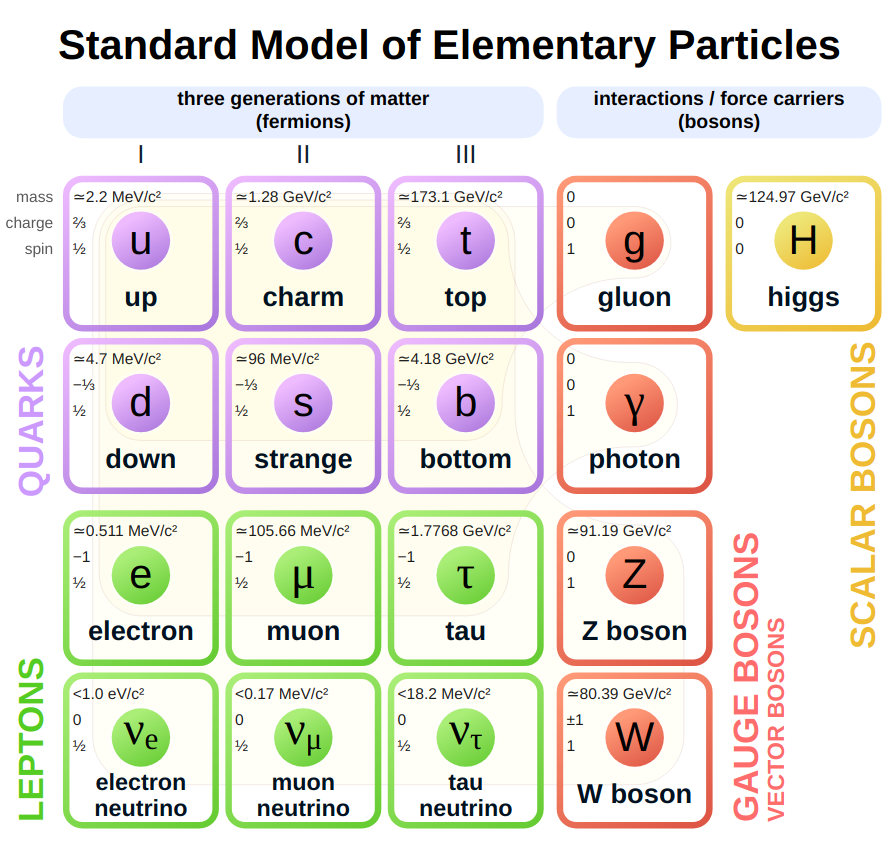
\includegraphics[width=0.8\textwidth]{content/images/SM.png}
            \caption*{Standard Model of particle physics \footnotemark{} }
          \end{figure}
        \end{column}
      \end{columns}
      \setcounter{footnote}{0}
      \stepcounter{footnote}{ \footnotetext{\url{https://en.wikipedia.org/wiki/Standard_Model}}}
\end{frame}

%\begin{frame}{Standard Model (SM)}
%  \begin{columns}
%    \begin{column}{0.5\textwidth}
%      \begin{itemize}
%        \item Spontaneous Symmetry Breaking
%        \begin{itemize}
%          \item $SU(3)_C \otimes SU(2)_L \otimes U(1)_\gamma \overset{SSB}{\rightarrow} SU(3)_C \otimes U(1)_\text{QED}$
%          \item Masses generated
%          \item Higgs-Boson
%        \end{itemize}
%      \end{itemize}
%    \end{column}
%    \begin{column}{0.5\textwidth}
%      \begin{figure}
%        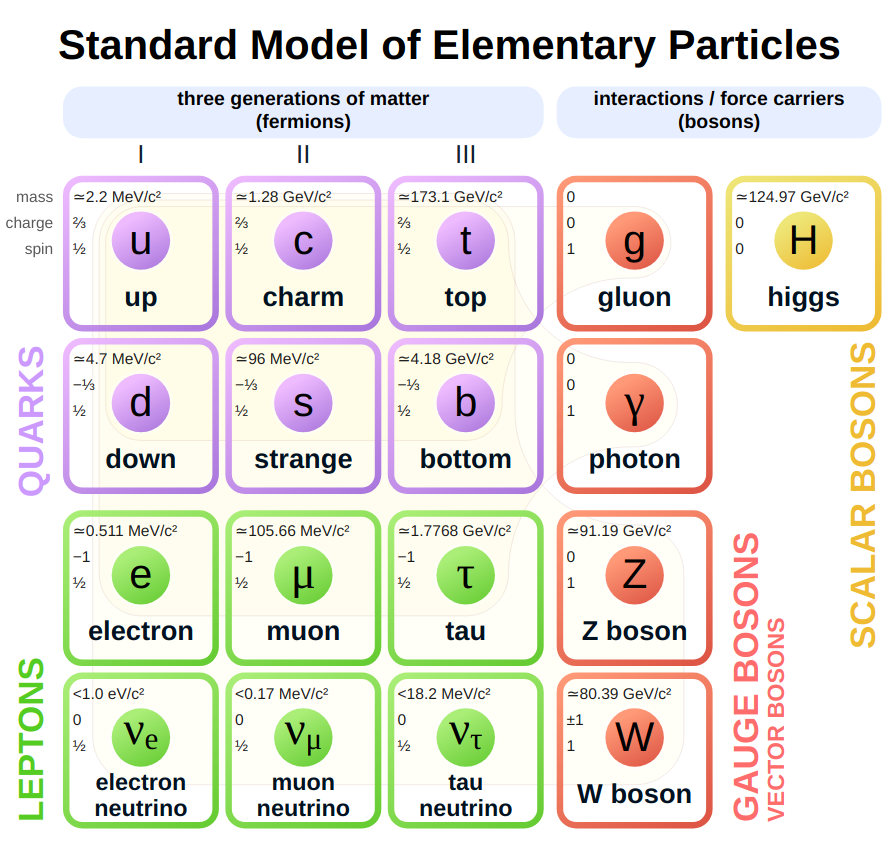
\includegraphics[width=0.8\textwidth]{content/images/SM.png}
%        \caption*{Standard Model of particle physics \footnotemark}
%      \end{figure}
%    \end{column}
%  \end{columns}
%  \footnotetext[1]{\url{https://en.wikipedia.org/wiki/Standard_Model}}
%\end{frame}

\begin{frame}{Leptons in the Standard Model}
  \begin{table}[]
    \begin{tabular}{lllll}
    \toprule 
    \textbf{Particle} & {\textbf{Q}$\:/\: \mathrm{e}$} & {\textbf{Mass}$\:/\: \mathrm{MeV}$} \\ 
    \midrule
     electron ($e$) & -1 &  0.511  \\
     neutrino ($\nu_e$) & 0 &  0  \\
     \midrule
     muon ($\mu$) & -1 &  105.66  \\
     neutrino ($\nu_\mu$) & 0 & 0 \\
     \midrule
     tau ($\tau$) & -1 & 1776.86 \\
     neutrino ($\nu_\tau$) & 0 & 0 \\
     \bottomrule
    \end{tabular}
\end{table}
\end{frame}


\begin{frame}{Electroweak Interaction}
    \setbeamercolor{normal text}{fg=gray,bg=}
    \setbeamercolor{alerted text}{fg=black,bg=}
    \usebeamercolor{normal text}
    \begin{columns}[T]
        \alert<1, 2>{ \begin{column}{0.5\textwidth}
            \begin{itemize}
                \item Charged Currents (CC)
                \item $W^\pm$-Boson interactions
                \begin{itemize}
                    \item left handed fermions
                    \item right handed anti-fermions
                    \item [\rightarrow] violates \textbf{C} and \textbf{P}
                \end{itemize}
                \item[] \includegraphics<2>[width=0.7\textwidth]{content/images/Wdecay1.png}
                        \includegraphics<3, 4>[width=0.7\textwidth]{content/images/Wdecay2.png}
            \end{itemize}
        \end{column}}
        %-------------%\textcolor
        \alert<3, 4>{\begin{column}{0.5\textwidth}
            \begin{itemize}
                \item Neutral Currents (NC)
                \item Z-Boson, Photon
                \begin{itemize}
                    \item decays into $l\bar{l}$
                    \item never observed: $Z \rightarrow e^{\pm} \mu^{\mp}$
                \end{itemize}
                \visible<4>{\item[] 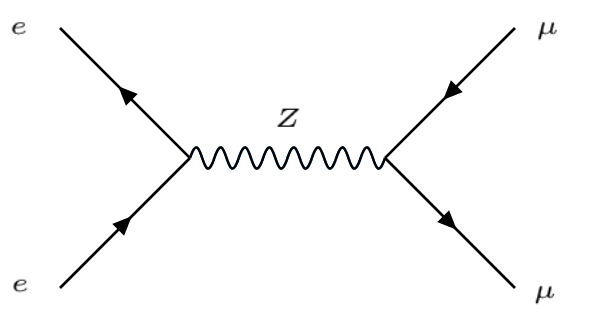
\includegraphics[width=0.8\textwidth]{content/images/Zdecay1.png}}
            \end{itemize}
        \end{column}}
    \end{columns}
\end{frame}

\begin{frame}{Charged Current \footnotemark }
    \begin{columns}
        \begin{column}{0.65\textwidth}
            In the SM, the lagrangian for the charged current is 
    \begin{equation*}
        \mathcal{L}_{CC} = \frac{g_1}{2 \sqrt{2}}  \left\{ W^{\dagger}_\mu \left[ \bar{u} \gamma^\mu (1-\gamma^5) d + \bar{\nu}_e \gamma^{\mu} (1-\gamma^5) e \right] \right\}
    \end{equation*}
    \begin{itemize}
        %\item $W^{\dagger}_{\mu} \hat{=} \text{boson field} $
        %\item $u, d \hat{=} \text{uptype, downtype quarks} $
        %\item $e \hat{=} \text{lepton}$
        %\item $\nu_e \hat{=} \text{neutrino}$
        \item $g_1 = \frac{e}{sin{(\theta_W)}}$
        \item independent of mass
    \end{itemize}
        \end{column}
        \begin{column}{0.35\textwidth}
            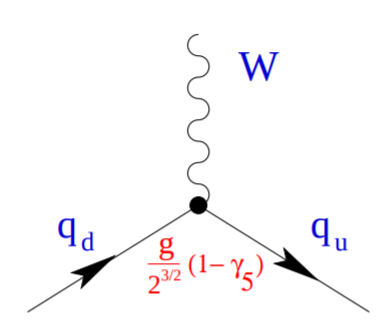
\includegraphics[width = 0.65\textwidth]{content/images/cc1.png}
            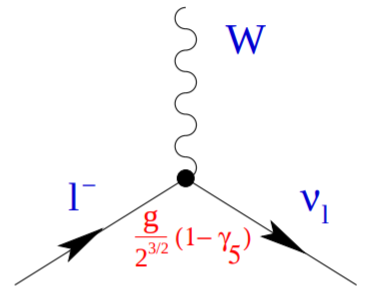
\includegraphics[width = 0.65\textwidth]{content/images/cc2.png}
        \end{column}
    \end{columns}
    \footnotetext{arXiv:hep-ph/0502010}
\end{frame}

\begin{frame}{Neutral Current}
    \begin{columns}
        \begin{column}{0.65\textwidth}
            In the SM, the lagrangian for the neutral current is 
    \begin{equation*}
        \mathcal{L}_\text{NC} = \frac{g_2}{2 \sin{(\theta_W)}} Z_\nu \sum_f \bar{f} \gamma^\mu \left( \nu_f - a_f \gamma_5 \right) f
    \end{equation*}
    \begin{itemize}
       % \item $a_f = T^f_3$
       % \item $ \nu_f = T^f_3( 1 - 4 |Q_f| \sin^2{(\theta_W)} ) $
        \item $ g_2 = \frac{e}{cos{(\theta_W)}} $
        \item independent of mass
    \end{itemize}
    \begin{figure}
        \centering
        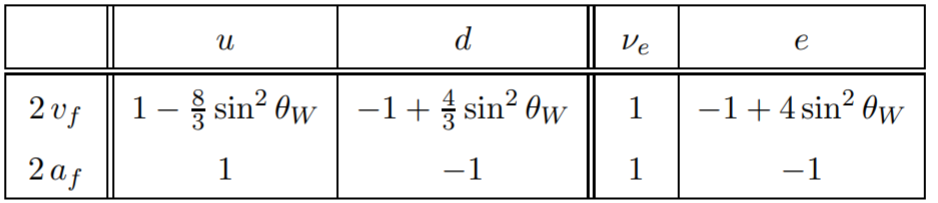
\includegraphics[width=0.8\textwidth]{content/images/nc_coublings.png}
    \end{figure}
        \end{column}
        \begin{column}{0.35\textwidth}
            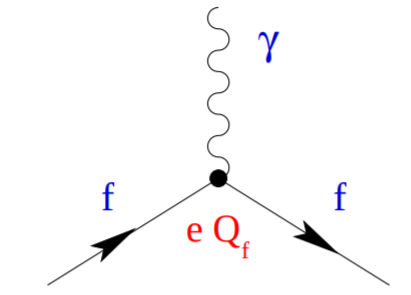
\includegraphics[width = 0.65\textwidth]{content/images/nc1.png}
            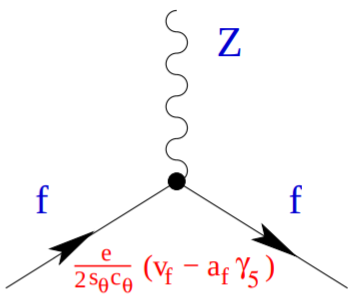
\includegraphics[width = 0.65\textwidth]{content/images/nc2.png}
        \end{column}
    \end{columns}
\end{frame}

\begin{frame}{Lepton Universality}
    \begin{itemize}
        \item charged and neutral currents studied:
        \begin{itemize}
            \item inpependent of mass
            \item constant coupling to all leptons
        \end{itemize}
        \item [\rightarrow] lepton flavour does not matter
    \end{itemize}
\end{frame}
\section{Lepton Universality Tests}
\subsection{The Electroweak Sector}
\frame{\tableofcontents[currentsection]}
    \begin{frame}{Partial Width of the Z-Boson}
        \begin{columns}
            \begin{column}{0.5\textwidth}
                \begin{itemize}
                    \item compare partial widths \rightarrow ratios
                    \begin{itemize}
                        \item no favoured flavour
                        \item [\rightarrow] expect ratios near 1
                    \end{itemize} 
                    \item measurements \footnotemark{} \footnotemark{} :
                    \begin{itemize}
                        \item [] <2, 3, 4 >$\frac{\Gamma_{Z \rightarrow \mu^+ \mu^-}}{\Gamma_{Z \rightarrow e^+ e^-}} = 1.0009 \pm 0.0028$
                        \item  []
                        \item [] <3, 4 > $\frac{\Gamma_{Z \rightarrow \tau^+ \tau^-}}{\Gamma_{Z \rightarrow e^+ e^-}} = 1.0019 \pm 0.0032$
                        \item []
                        \item [] <4>$\frac{\Gamma_{Z \rightarrow \mu^+ \mu^-}}{\Gamma_{Z \rightarrow e^+ e^-}} = 0.9974 \pm 0.0050$
                        %
                    \end{itemize}
                \end{itemize}
            \end{column}
            \begin{column}{0.5\textwidth}
                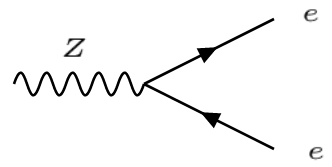
\includegraphics[width = 0.42\textwidth]{content/images/Zdecay_ee.png} \\
                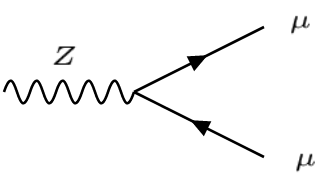
\includegraphics[width = 0.42\textwidth]{content/images/Zdecay_mumu.png} \\
                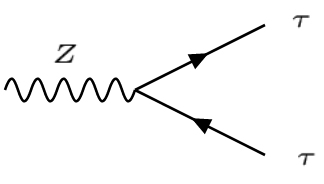
\includegraphics[width = 0.42\textwidth]{content/images/Zdecay_tautau.png}
            \end{column}
        \end{columns}
        \footnotetext{arXiv:hep-ex/0509008}
        \footnotetext{arXiv:1612.03016}
    \end{frame}
    \begin{frame}{Partials Widths of the $W^{\pm}$-Boson}
        \begin{columns}
            \begin{column}{0.5\textwidth}
              \begin{itemize}
                \item compare partial widths \rightarrow ratios
                \begin{itemize}
                    \item no favoured flavour
                    \item [\rightarrow] expect ratios near 1
                \end{itemize} 
                \item measurements \footnotemark{} :
                \begin{itemize}
                    \item [] < 2, 3, 4, 5> $\frac{\Gamma_{W \rightarrow \tau^- \bar{\nu}_\tau}}{\Gamma_{W \rightarrow e^- \bar{\nu}_e }} = 1.063 \pm 0.027$
                    \item  []
                    \item [] < 3, 4, 5> $\frac{\Gamma_{W \rightarrow \tau^- \bar{\nu}_\tau}}{\Gamma_{W \rightarrow \mu^- \bar{\nu}_\mu }} = 1.070 \pm 0.026$
                    \item []
                    \item [] <4, 5>$\frac{2\Gamma_{W \rightarrow \tau^- \bar{\nu}_\tau}}{\Gamma_{W \rightarrow \mu^- \bar{\nu}_\mu } + \Gamma_{W \rightarrow e^- \bar{\nu}_e }} = 1.066 \pm 0.025$
                \end{itemize}
                \item <5> $\approx 2.3 \sigma $ deviation!
            \end{itemize}
            \end{column}
            \begin{column}{0.5\textwidth}
                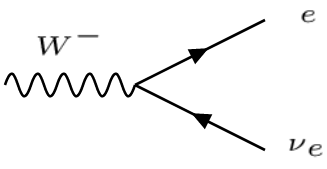
\includegraphics[width = 0.42\textwidth]{content/images/Wdecay_e.png} \\
                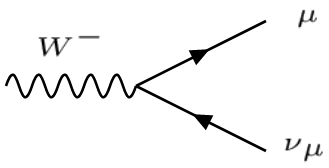
\includegraphics[width = 0.42\textwidth]{content/images/Wdecay_mu.png} \\
                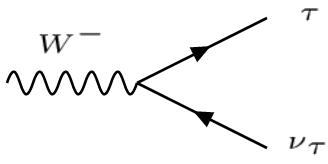
\includegraphics[width = 0.42\textwidth]{content/images/Wdecay_tau.png}
            \end{column}
        \end{columns}
        \footnotetext{arXiv:1302.3415}
    \end{frame}

    \begin{frame}{Difficulty: tau reconstruction}
        \begin{columns}
            \begin{column}{0.45\textwidth}
                \begin{itemize}
                    \item channels
                    \begin{itemize}
                        \item $ \tau_l$
                        \item $ \tau_{\text{had}}$
                    \end{itemize}
                    \visible<2, 3, 4>{ \item $\tau_{\text{had}}$ means a hadronically decaying tau-leptons
                    \begin{itemize}
                        \item no visible jets
                        \item decay products form pions 
                    \end{itemize}}
                    \visible<3, 4>{
                    \item $\tau_{\text{lep}}$ means leptonically decaying tau-leptons
                    \begin{itemize}
                        \item two neutrinos \textrightarrow difficult to reconstruct
                        \item only leptons (e, $\mu$) visible
                    \end{itemize}}
                    \item <4> may be cause of deviation
                \end{itemize}
            \end{column}
            \begin{column}{0.55\textwidth}
                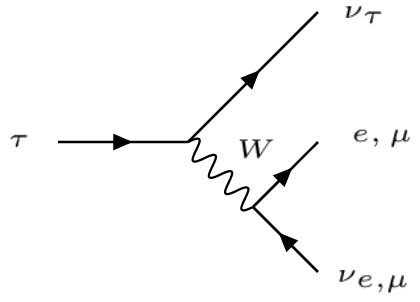
\includegraphics[scale=0.3]{content/feynman/png/tau_lep.png}
                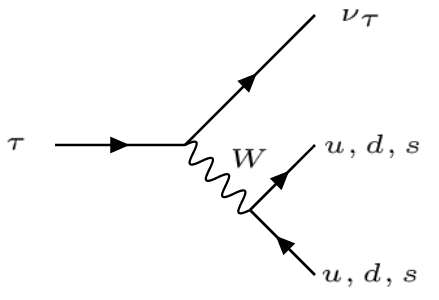
\includegraphics[scale=0.3]{content/feynman/png/tau_had.png}
            \end{column}
        \end{columns}
    \end{frame}

    \begin{frame}{Branching Ratios of the $W^{\pm}$-Boson}
        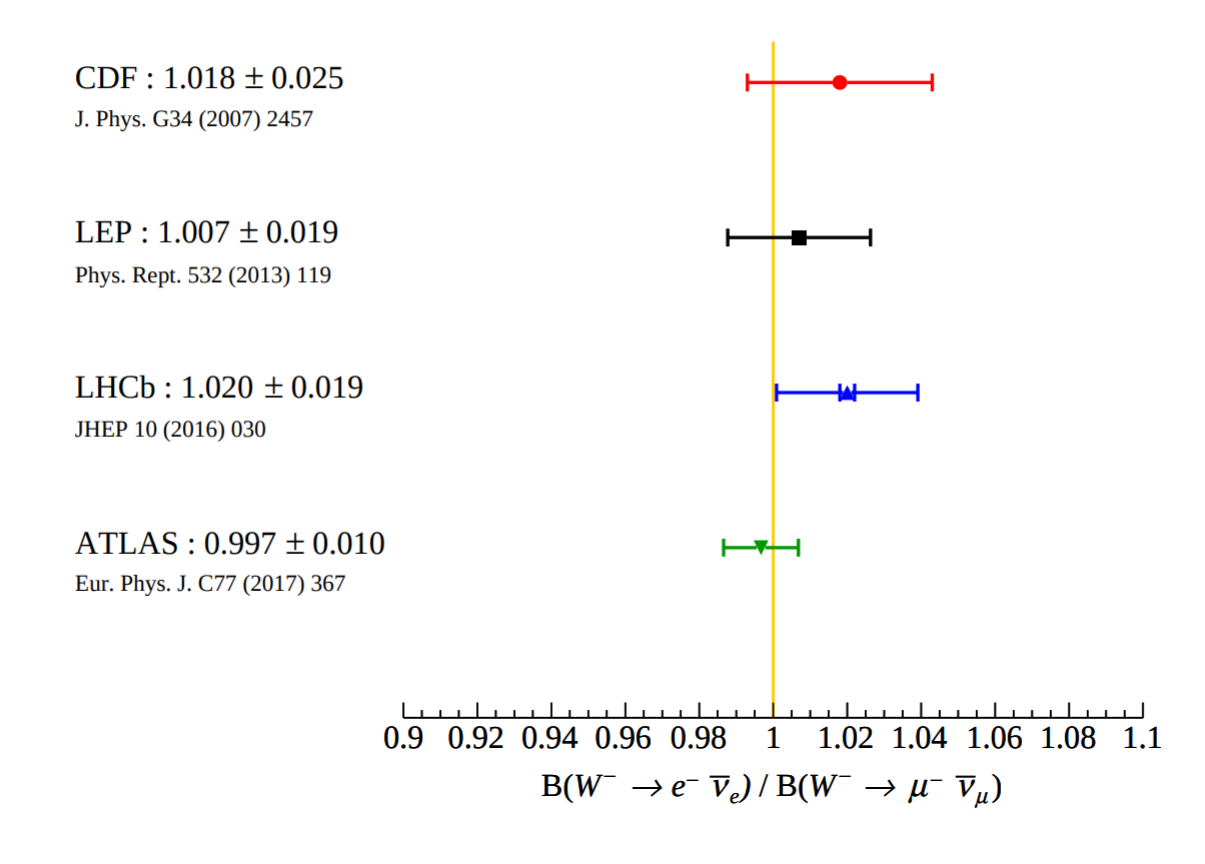
\includegraphics[width=0.7\textwidth]{content/images/BR_W.png}
    \end{frame}

\subsection{Pseudoscalar Mesons}
%\frame{\tableofcontents[currentsection]}
\begin{frame}{Pseudoscalar Mesons}
    \begin{columns}[T]
        \begin{column}{0.7\textwidth}
            \begin{itemize}
                \item study decay of $\pi^-$
                \begin{itemize}
                    \item composed of $d, \bar{u} $
                    \item Spin 0
                    \visible<2, 3, 4, 5>{\item [\rightarrow] consider helicity}
                \end{itemize}
                \item 
                 \begin{align*}
                    \left(\frac{\Gamma_{\pi^- \rightarrow e^- \bar{\nu}_e}}{\Gamma_{\pi^- \rightarrow \mu^- \bar{\nu}_\mu}} \right)^{SM} \only<1, 2>{\neq 1 } \visible<3, 4, 5>{ &= \left(\frac{M_e}{M_\mu} \right)^2 \frac{M^2_\pi - M^2_e}{M^2_\pi - M^2_\mu}(1 +\delta_\text{QED} )  \\
                    \visible<4, 5>{ &= (1.2352 \pm 0.0001)\cdot 10^{-4}} }
                \end{align*}
               \visible<5>{ \item measured :
                \begin{itemize}
                    \item $\frac{\Gamma_{\pi^- \rightarrow e^- \bar{\nu}_e}}{\Gamma_{\pi^- \rightarrow \mu^- \bar{\nu}_\mu}} = (1.230 \pm 0.004) \cdot 10^{-4} $
                \end{itemize}}
            \end{itemize}
        \end{column}
        %------------%
        \begin{column}{0.4\textwidth}
            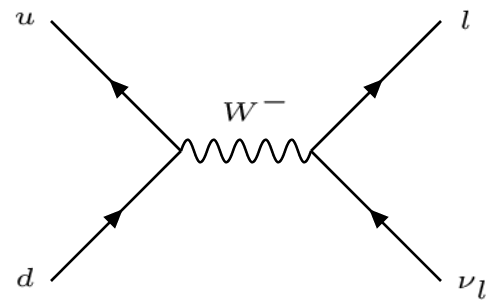
\includegraphics[width = 0.7\textwidth]{content/images/pi_l.png} \\
            \visible<2, 3, 4, 5>{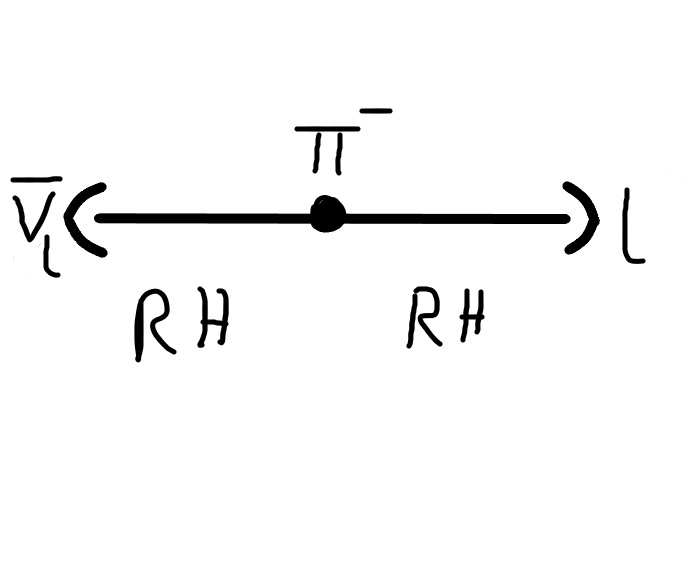
\includegraphics[width = 0.8\textwidth]{content/images/pi_hel.png}} 
            %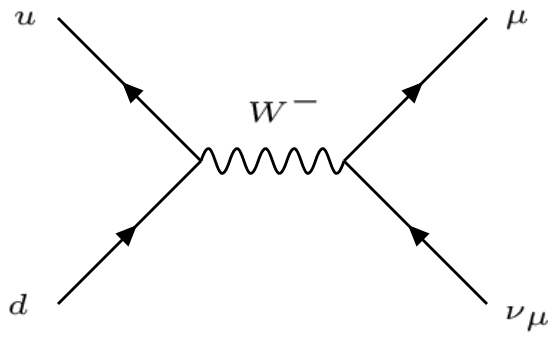
\includegraphics[width = 0.7\textwidth]{content/images/pi_mu.png} 
        \end{column}
    \end{columns}
    
\end{frame}

\subsection{Meson Mixing}
\begin{frame}{$R_{K}$ and $R_{K^*}$}
    \begin{columns}
        \begin{column}{0.5\textwidth}
            \begin{itemize}
                \item anomalies in $\bar{B}^{0} \rightarrow \bar{H} l \bar{l}$ 
                \begin{itemize}
                    \item $H = K, K^*$
                \end{itemize} 
                \item <2, 3, 4> $R_{K} = \frac{ \displaystyle \int_{q^2_{min}}^{q^2_{max}} \frac{\symup{d}\mathcal{B} [ B \rightarrow H \mu^+ \mu^- ] } {\symup{d}q^2} } {\displaystyle \int_{q^2_{min}}^{q^2_{max}} \frac{\symup{d}\mathcal{B} [ B \rightarrow H e^+ e^- ] } {\symup{d}q^2}} \stackrel{!}{=} 1$ 
                \item <3, 4> LHCb \footnotemark:
                \begin{itemize}
                    \item <3, 4> $R_K = 0.745 \substack{+0.090 \\ -0.074} \pm 0.036$
                    \item <3, 4> $R_{K^*} = 0.69 \substack{+0.11 \\ -0.07} \pm 0.005$
                \end{itemize}
                \item <4> Potential lepton flavour-violation ($2.6 \sigma$)
                \item <4> Leptoquarks may be the answer to this!
            \end{itemize}
        \end{column}
        \begin{column}{0.5\textwidth}
            \begin{itemize}
                \item []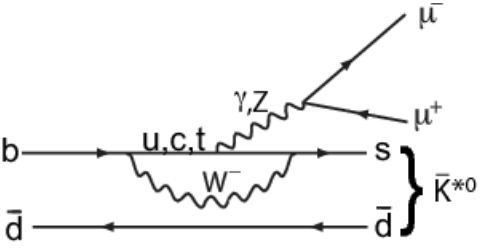
\includegraphics[scale=0.25]{content/feynman/png/BtoK1.png}
                \item []
                \item []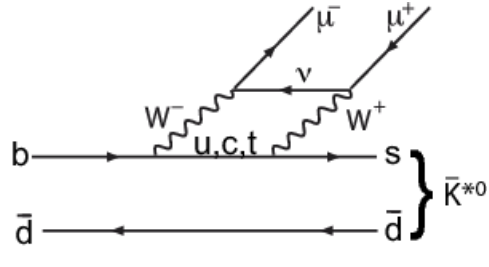
\includegraphics[scale=0.25]{content/feynman/png/BtoK2.png}
            \end{itemize}
        \end{column}
    \end{columns}
    \footnotetext{arXiv:1406.6482}
\end{frame}


\section{Beyond Standard Model: Leptoquarks}
\frame{\tableofcontents[currentsection]}
\begin{frame}{Beyond the Standard Modell: Leptoquarks}
    \begin{columns}
        \begin{column}{0.55\textwidth}
            \begin{itemize}
                \item Theories: supersymmetry, grand unification
                \begin{itemize}
                    \item imply: scalars with colour and different quantum numbers
                    \item [\rightarrow] Leptoquarks
                \end{itemize}
            \end{itemize}
            \begin{itemize}
                \item <2-> Leptoquarks (LQs)
                    \begin{itemize}
                        \item <3-> spin 0 or spin 1
                        \item <3->lepton number (L) $\neq$ 0
                        \item <3->baryon number (B) $\neq$ 0
                        \item <4->mass $\mathcal{O}\left( TeV \right)$
                        \item <5->Three generations of LQs:
                        \begin{itemize}
                            \item Generation X of LQs couples to Generation X of the SM
                            \item [] $X \in \{1, 2, 3 \}$
                        \end{itemize}
                        \item <6->Coupling across generations possible
                    \end{itemize}
            \end{itemize}
        \end{column}
        \begin{column}{0.45\textwidth}
            \begin{itemize}
                \item [] Possible Leptoquarks and their quantum numbers\footnotemark{}
            \end{itemize}
            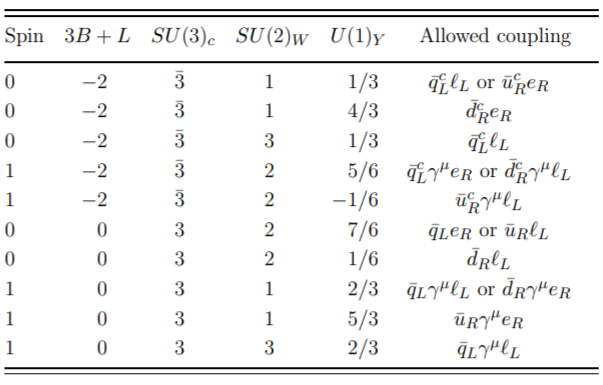
\includegraphics[scale=0.32]{content/images/LQ-Table.PNG}
        \end{column}
    \end{columns}
    \footnote{Phys. Lett. B 191 (1987) 442}
\end{frame}

\begin{frame}{How LQs can contribute to $R_{K}$ and $R_{K^*}$ }
    \begin{columns}
        \begin{column}{0.6\textwidth}
            \begin{itemize}
                \item $R_{K} < 1$
                \begin{itemize}
                    \item < 2-> too many electrons
                    \item < 2-> too few muons
                    \item < 2-> combination of both?
                \end{itemize}
                \item < 3->LQs have tcouple differently to different lepton generations
            \end{itemize}
        \end{column}
        \begin{column}{0.4\textwidth}
            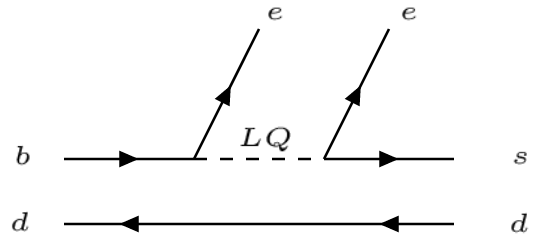
\includegraphics[width=0.7\textwidth]{content/images/LQ_ee.png}
            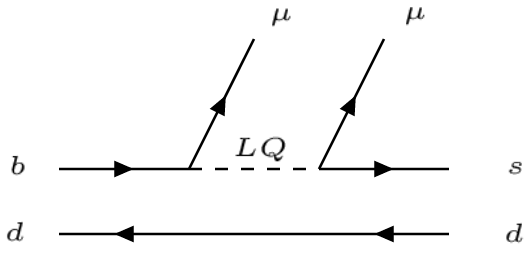
\includegraphics[width=0.7\textwidth]{content/images/LQ_mumu.png}
        \end{column}
    \end{columns}
\end{frame}

\section{Conclusion}
\frame{\tableofcontents[currentsection]}
\begin{frame}{Conclusion}
    \begin{itemize}
        \item Lepton Universality:
        \begin{itemize}
            \item Interaction of gauge bosons and leptons is flavour-independent \medskip
        \end{itemize}
        \item Most tests correspond to LU \medskip
        \item $R_{K}$ and $R_{K^*}$: $2.6 \sigma$ deviaton \medskip
        \item Leptoquarks may explain $R_{K}$ and $R_{K^*}$ \medskip
    \end{itemize}
\end{frame}
\end{document}
